%   File: Golfer.tex
% Author: Adam Leeper
%------------------------------------------------------------------------------
%\\[0.45pc]
\providecommand{\isolatedBuild}[1]{#1}% Fallback definition to build normally.
\isolatedBuild{
  \documentclass[11pt,letterpaper]{book}
  %\documentclass[11pt,letterpaper]{book}

% aleeper: I think these are needed for Paul's macros?
\usepackage{epsfig}
\usepackage{epstopdf}

%\makeatletter
%\typeout{The import path is \import@path}
%\makeatother

\usepackage{import}

\subimport{./}{packagesMitiguy.sty}
\subimport{./}{macrosMitiguy.tex}
\subimport{./}{PageStylesMitiguy.tex}
\subimport{./}{macrosLeeper.tex}
   % Found via TEXINPUTS environment variable.
  \isolatedBuildHeader{Rotation Matrices}
                      {3D Visual Thinking (draw/think 3D)
                        - for disordered unit vectors.}
}
%%%
%%%
%%%
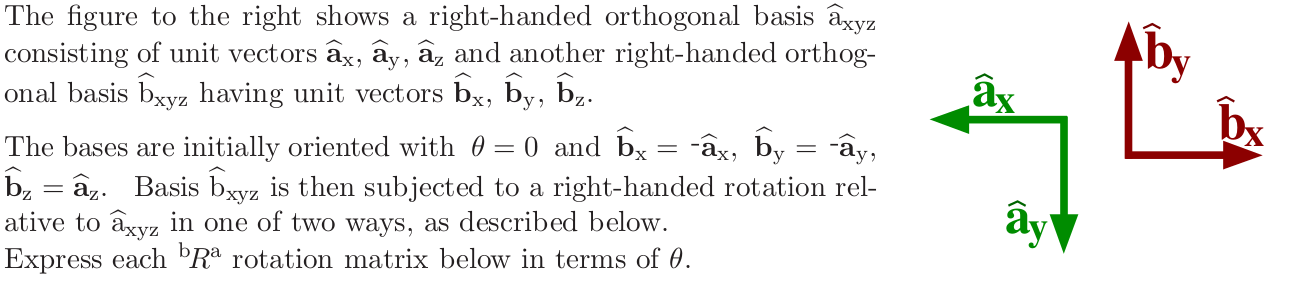
\includegraphics[width=0.93\textwidth]{disorderly_vectors1.png}

\textbf{(a)} To help you get started, \textbf{first} form the rotation matrix when $\theta = 0$, which is the configuration shown.
\\[0.0pc]
\hspace*{0.7cm}(The matrix contains only integers.)
\\[0.5pc]
\hspace*{1cm} {\large \rotationTableEmpty{b}{a}{\hspace*{1cm}}}
\\[1.0pc]
%
\textbf{(b)} Now form matrices for the rotations described, in terms of $\theta$.
\\[0.0pc]
\hspace*{0.7cm}\textbf{Hint:} Hug-rule won't work; instead \textbf{\underline{draw}} and use \textbf{definitions}.
\\[0.0pc]
\hspace*{0.7cm}\textbf{Hint:} If you plug $\theta = 0$ into your results for (b), you should get the matrix in (a).
\\[0.0pc]
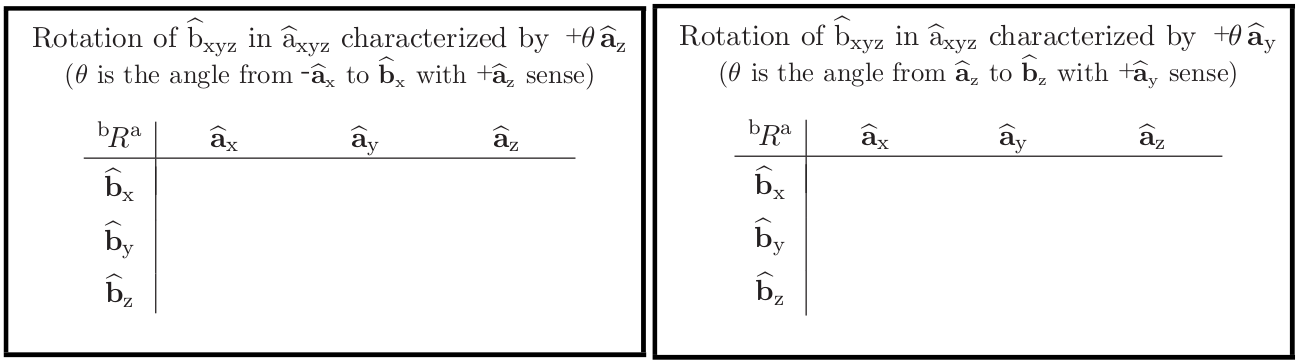
\includegraphics[width=1.0\linewidth]{disorderly_vectors2.png}
%
\isolatedBuildFooter